\documentclass[letterpaper, 12pt]{math}

\usepackage{tikz}

\title{Multivariable and Vector Calculus}
\author{Alvin Lin}
\date{August 2017 - December 2017}

\begin{document}

\maketitle

\section*{Functions of Several Variables}
A function of a single variable:
\begin{center}
  \begin{tikzpicture}
    \draw (0,0) -- node[below] {x} (2,0) -- node[right] {x} (2,2) --
      (0,2) -- (0,0);
  \end{tikzpicture}
\end{center}
\[ A(x) = x^2 \]
A function of two variables:
\begin{center}
  \begin{tikzpicture}
    \draw (0,0) -- node[below] {x} (4,0) -- node[right] {y} (4,2) --
      (0,2) -- (0,0);
  \end{tikzpicture}
\end{center}
\[ A(x,y) = xy \]
Even for functions of many variables, they still have properties such as domain
and range.
\[ f(x,y) = \frac{1}{\sqrt{1-x^2-y^2}} \]
Domain:
\[ 1-x^2-y^2 > 0 \therefore x^2+y^2 < 1 \]
Range:
\[ [1,\infty) \]

\subsubsection*{Example}
Find the domain of the function:
\[ f(x,y) = \frac{\ln(2-x)}{\sqrt{x-3y}} \]
\begin{align*}
  2-x &> 0 \\
  &\equiv x < 2\\
  x-3y &> 0 \\
  &\equiv y < \frac{x}{3}
\end{align*}
\begin{center}
  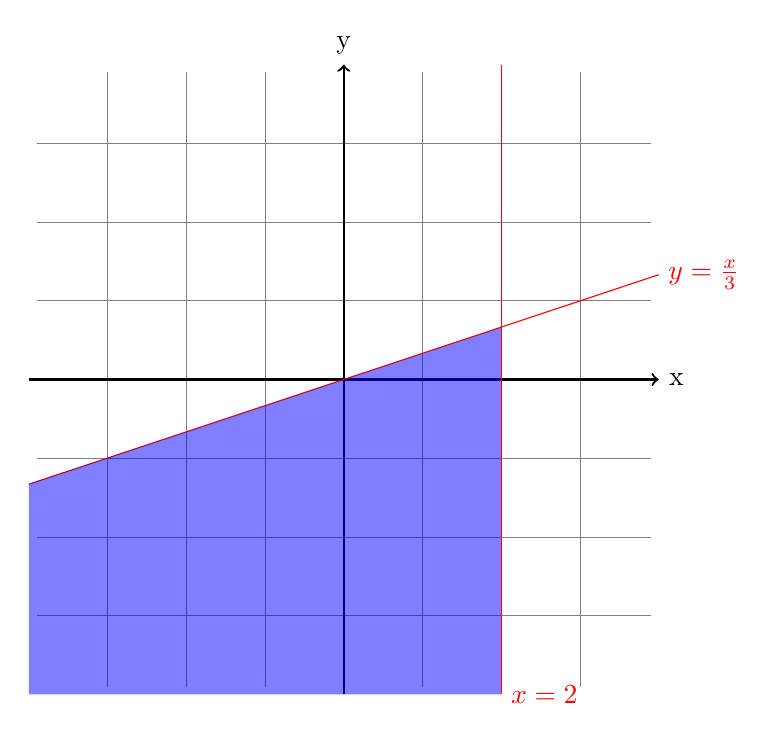
\begin{tikzpicture}
    \draw[step=1cm,gray,very thin] (-3.9,-3.9) grid (3.9,3.9);
    \draw[thick,->] (-4,0) -- (4,0) node[right] {x};
    \draw[thick,->] (0,-4) -- (0,4) node[above] {y};
    \draw[red] (2,4) -- (2,-4) node[right] {\( x = 2 \)};
    \draw[red] (-4,-1.33) -- (4,1.33) node[right] {\( y = \frac{x}{3} \)};
    \fill[opacity=0.5,blue] (-4,-1.33) -- (2,0.66) -- (2,-4) -- (-4,-4) --
      cycle;
  \end{tikzpicture}
\end{center}

\begin{center}
  You can find all my notes at \url{http://omgimanerd.tech/notes}. If you have
  any questions, comments, or concerns, please contact me at
  alvin@omgimanerd.tech
\end{center}

\end{document}
